../cictikz/src/cictikz/data/tex/cictikz_preamble.tex

% TFE4188 from first thoughts to fourth-of-four. Above the axis: the one thing
% I added that year. Below: what the students got out of it, one square per
% project group, filled if the group reached a tapeout.
%
% Group counts are the analogicus repos with a contributor other than me:
% cnr_gr02..06 (5), jnw_gr01..07 (7), lelo_gr01..04 (4). The other gr repos
% in each series were created but never used by a group.
%
% 2020 is planning only -- the course did not run. Dates from the original
% course-plan git repo (data/2019/NTNU/archive/tfe41xx_aic/admin/plan):
% "First thoughts on course" 2020-01-03, plan reviewed 2020-02-14. The 2021
% teaching was TFE4152, not this course. TFE4188 first ran spring 2022.

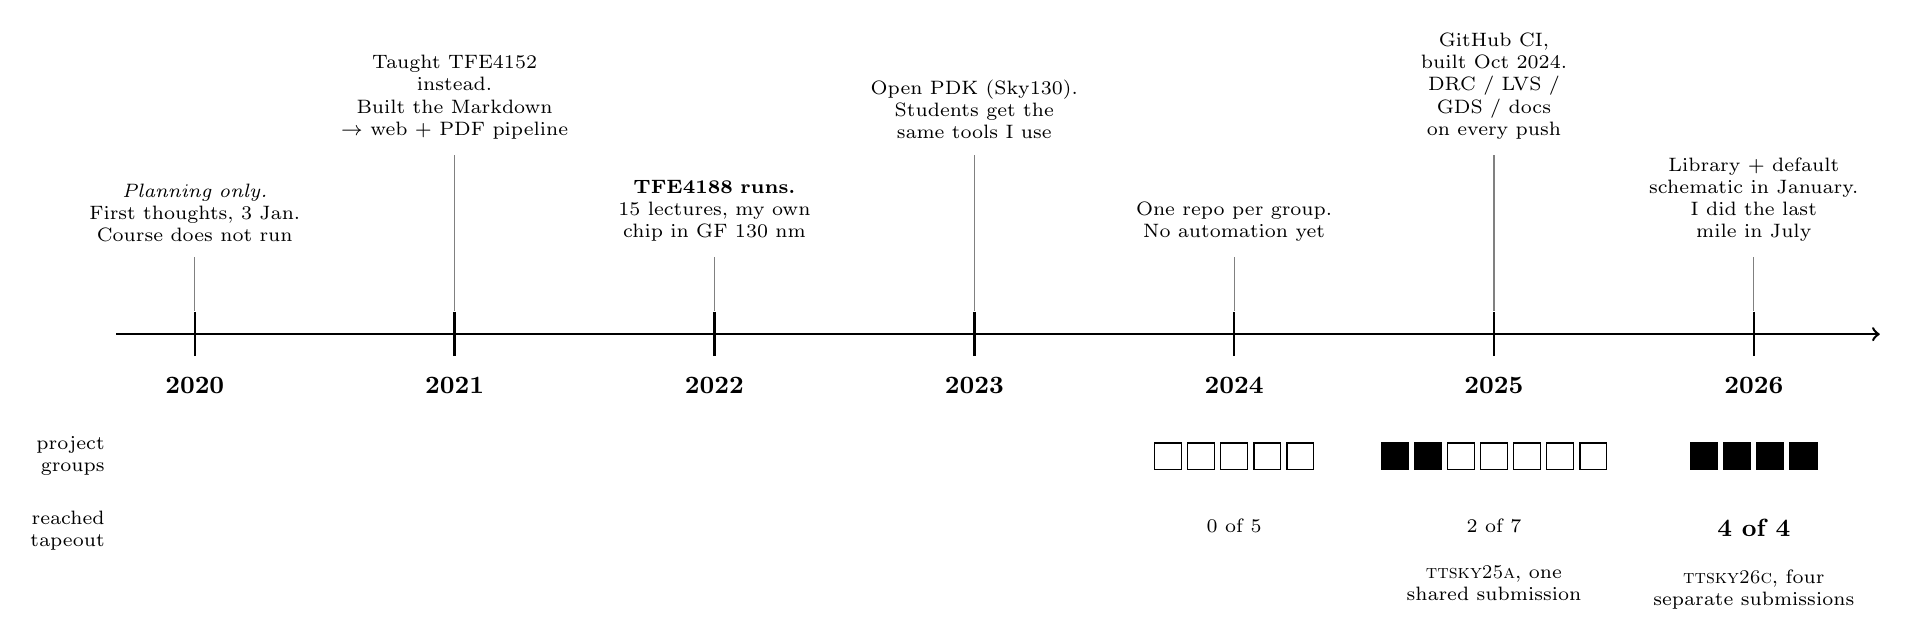
\begin{tikzpicture}[line width=0.5pt]

  \tikzset{
    yr/.style   = {font=\small\bfseries},
    add/.style  = {font=\scriptsize, align=center, text width=2.9cm,
                   inner sep=2pt},
    note/.style = {font=\scriptsize, align=center, inner sep=1pt},
    lead/.style = {line width=0.4pt, gray},
    chip/.style = {draw, line width=0.5pt, minimum size=0.34cm, inner sep=0pt},
    done/.style = {chip, fill=black},
    todo/.style = {chip, fill=white},
  }

  \def\dx{3.3}                     % cm per year

  % ---- axis -------------------------------------------------------------
  \draw[line width=0.9pt,->] (-1.0,0) -- (21.4,0);

  \foreach \i/\y in {0/2020, 1/2021, 2/2022, 3/2023, 4/2024, 5/2025, 6/2026} {
    \draw[line width=0.9pt] (\i*\dx,-0.28) -- (\i*\dx,0.28);
    \node[yr,anchor=north] at (\i*\dx,-0.42) {\y};
  }

  % ---- what I added, above the axis -------------------------------------
  \foreach \i/\h/\t in {%
    0/1.1/{\emph{Planning only.}\\First thoughts, 3 Jan.\\Course does not run},
    1/2.4/{Taught TFE4152 instead.\\Built the Markdown\\$\rightarrow$ web + PDF pipeline},
    2/1.1/{\textbf{TFE4188 runs.}\\15 lectures, my own\\chip in GF 130 nm},
    3/2.4/{Open PDK (Sky130).\\Students get the\\same tools I use},
    4/1.1/{One repo per group.\\No automation yet},
    5/2.4/{GitHub CI, built Oct 2024.\\DRC / LVS / GDS / docs\\on every push},
    6/1.1/{Library + default\\schematic in January.\\I did the last mile in July}%
  }{
    \draw[lead] (\i*\dx,0.3) -- (\i*\dx,\h-0.12);
    \node[add,anchor=south] at (\i*\dx,\h) {\t};
  }

  % ---- what the students did, below the axis -----------------------------
  \node[note,anchor=east,align=right] at (-1.1,-1.55)
    {project\\groups};
  \node[note,anchor=east,align=right] at (-1.1,-2.5)
    {reached\\tapeout};

  % 2024: five groups, none taped out
  \foreach \k in {0,...,4} {
    \pgfmathsetmacro{\xx}{4*\dx + (\k-2)*0.42}
    \node[todo] at (\xx,-1.55) {};
  }
  \node[note,anchor=north] at (4*\dx,-2.3) {0 of 5};

  % 2025: seven groups, two of them taped out on ttsky25a
  \foreach \k in {0,...,6} {
    \pgfmathsetmacro{\xx}{5*\dx + (\k-3)*0.42}
    \ifnum\k<2 \node[done] at (\xx,-1.55) {}; \else
                \node[todo] at (\xx,-1.55) {}; \fi
  }
  \node[note,anchor=north] at (5*\dx,-2.3) {2 of 7};
  \node[note,anchor=north] at (5*\dx,-2.9) {\textsc{ttsky25a}, one\\shared submission};

  % 2026: four groups, all four taped out on ttsky26c
  \foreach \k in {0,...,3} {
    \pgfmathsetmacro{\xx}{6*\dx + (\k-1.5)*0.42}
    \node[done] at (\xx,-1.55) {};
  }
  \node[note,anchor=north,font=\small\bfseries] at (6*\dx,-2.3) {4 of 4};
  \node[note,anchor=north] at (6*\dx,-2.95) {\textsc{ttsky26c}, four\\separate submissions};

\end{tikzpicture}
\end{document}
